

\begin{article}





\title{Taming PITCHf/x Data with \pkg{XML2R} and \pkg{pitchRx}}


\author{by Carson Sievert}

\maketitle
\abstract{\pkg{XML2R} is a framework that reduces the effort required to transform
XML content into tables in a way that preserves parent to child relationships.
\pkg{pitchRx} applies \pkg{XML2R}'s grammar for XML manipulation
to Major League Baseball Advanced Media (MLBAM)'s Gameday data. With
\pkg{pitchRx}, one can easily obtain and store Gameday data in a
remote database. The Gameday website hosts a wealth of XML data, but
perhaps most interesting is PITCHf/x. Among other things, PITCHf/x
data can be used to recreate a baseball's flight path from a pitcher's
hand to home plate. With \pkg{pitchRx}, one can easily create animations
and interactive 3D scatterplots of the baseball's flight path. PITCHf/x
data is also commonly used to generate a static plot of baseball locations
at the moment they cross home plate. These plots, sometimes called
\dfn{strike-zone plots}, can also refer to a plot of event probabilities
over the same region. \pkg{pitchRx} provides an easy and robust way
to generate strike-zone plots using the \pkg{ggplot2} package. }


\section{Introduction}


\subsection{What is PITCHf/x?}

PITCHf/x is a general term for a system of cameras which tracks the
flight of a baseball with a series of 3D measurements. These measurements
define a baseball's flight path from a pitcher's hand to home plate.%
\footnote{A \dfn{pitcher} throws a ball to the opposing \dfn{batter}, who
stands besides home plate and tries to hit the ball into the field
of play.%
} A best fitting parametric curve is fit to these measurements under
the assumption of constant acceleration \citep{patent}. There are
studies that suggest that this assumption is quite reasonable -- especially
for non-knuckleballs \citep{trajecoryAnalysis}. In other words, the
smoothed flight paths are often a reasonable approximation (within
a couple of inches) of the real path. The parameters used to fit this
curve are made available in XML format on a publicly accessible website.
This website, maintained by MLBAM, also hosts a wealth of other baseball
related data used to inform MLB's Gameday webcast in near real time.


\subsection{Why is PITCHf/x important?}

On the business side of baseball, using statistical analysis to scout
and evaluate players has become mainstream. When PITCHf/x was first
introduced, \citep{slate} proclaimed it as, \begin{quote} ``The new technology that will change statistical analysis [of baseball] forever.'' \end{quote}
PITCHf/x has yet to fully deliver this claim, partially due to the
difficulty in accessing and deriving insight from the large amount
of complex information. By providing better tools to collect and visualize
this data, \CRANpkg{pitchRx} makes PITCHf/x analysis more accessible
to the general public.


\subsection{PITCHf/x applications}

PITCHf/x data is and can be used for many different projects. It can
also complement other baseball data sources, which poses an interesting
database management problem. Statistical analysis of PITCHf/x data
and baseball in general has become so popular that it has helped expose
statistical ideas and practice to the general public. If you have
witnessed television broadcasts of MLB games, you know one obvious
application of PITCHf/x is locating pitches in the strike-zone as
well as recreating flight trajectories, tracking pitch speed, etc.
Some well-known and statistically intriguing problems related to PITCHf/x
include: classifying pitch types, predicting pitch sequences, and
clustering pitchers with similar tendencies \citep{curve}.


\subsection[{Contributions of pitchRx and XML2R]{Contributions of \pkg{pitchRx} and \pkg{XML2R}}

\pkg{pitchRx} has two main focuses \citep{pitchRx}. The first focus
is to provide easy access to Gameday data. Not only is \pkg{pitchRx}
helpful for collecting this data in bulk, but it has served as a helpful
teaching and research aide (\url{http://baseballwithr.wordpress.com/}
is one such example). Methods for collecting Gameday data existed
prior to \pkg{pitchRx}; however, these methods are not easily extensible
and require juggling technologies that may not be familiar or accessible
\citep{database}. Moreover, these working environments are less desirable
than R for data analysis and visualization. Since \pkg{pitchRx} is
built upon \CRANpkg{XML2R}'s united framework, it can be easily modified
and/or extended \citep{XML2R}. For this same reason, \pkg{pitchRx}
serves as a model for building customized XML data collection tools
with \pkg{XML2R}.

The other main focus of \pkg{pitchRx} is to simplify the process
creating popular PITCHf/x graphics. Strike-zone plots and animations
made via \pkg{pitchRx} utilize the extensible \CRANpkg{ggplot2}
framework as well as various customized options \citep{ggplot2}.
\pkg{ggplot2} is a convenient framework for generating strike-zone
plots primarily because of its facet schema which allows one to make
visual comparisons across any combination of discrete variable(s).
Interactive 3D scatterplots are based on the \CRANpkg{rgl} package
and useful for gaining a new perspective on flight trajectories \citep{rgl}.


\section{Getting familiar with Gameday}

Gameday data is hosted and made available for free thanks to MLBAM
via \url{http://gd2.mlb.com/components/game/mlb/}.%
\footnote{Please be respectful of this service and store any information after
you extract it instead of repeatedly querying the website. Before
using any content from this website, please also read the \href{http://gdx.mlb.com/components/copyright.txt}{copyright}.%
} From this website, one can obtain many different types of data besides
PITCHf/x. For example, one can obtain everything from \href{http://gd2.mlb.com/components/game/mlb/year_2013/month_07/day_16/gid_2013_07_16_aasmlb_nasmlb_1/media/instadium.xml}{structured media metadata}
to \href{http://gd2.mlb.com/components/game/mlb/twitter/anaInsiderTweets.xml}{insider tweets}.
In fact, this website's purpose is to serve data to various \url{http://mlb.com}
web pages and applications. As a result, some data is redundant and
the format may not be optimal for statistical analysis. For these
reasons, the \code{scrape} function is focused on retrieving data
that is useful for PITCHf/x analysis and providing it in a convenient
format for data analysis. 

Navigating through the MLBAM website can be overwhelming, but it helps
to recognize that a homepage exists for nearly every day and every
game. For example, \url{http://gd2.mlb.com/components/game/mlb/year_2011/month_02/day_26/}
displays numerous hyperlinks to various files specific to February
26th, 2011. On this page is a hyperlink to \href{http://gd2.mlb.com/components/game/mlb/year_2011/month_02/day_26/miniscoreboard.xml}{miniscoreboard.xml}
which contains information on every game played on that date. This
page also has numerous hyperlinks to game specific pages. For example,
\href{http://gd2.mlb.com/components/game/mlb/year_2011/month_02/day_26/gid_2011_02_26_phimlb_nyamlb_1/}{gid\_2011\_02\_26\_phimlb\_nyamlb\_1/}
points to the homepage for that day's game between the NY Yankees
and Philadelphia Phillies. On this page is a hyperlink to the \href{http://gd2.mlb.com/components/game/mlb/year_2011/month_02/day_26/gid_2011_02_26_phimlb_nyamlb_1/players.xml}{players.xml}
file which contains information about the players, umpires, and coaches
(positions, names, batting average, etc.) coming into that game. 

Starting from a particular game's homepage and clicking on the \href{http://gd2.mlb.com/components/game/mlb/year_2011/month_02/day_26/gid_2011_02_26_phimlb_nyamlb_1/inning/}{inning/}
directory, we \emph{should} see another page with links to the \href{http://gd2.mlb.com/components/game/mlb/year_2011/month_02/day_26/gid_2011_02_26_phimlb_nyamlb_1/inning/inning_all.xml}{inning\_all.xml}
file and the \href{http://gd2.mlb.com/components/game/mlb/year_2011/month_02/day_26/gid_2011_02_26_phimlb_nyamlb_1/inning/inning_hit.xml}{inning\_hit.xml}
file. If it is available, the \code{inning\_all.xml} file contains
the PITCHf/x data for that game. It's important to note that this
file won't exist for some games, because some games are played in
venues that do not have a working PITCHf/x system in place. This is
especially true for preseason games and games played prior to the
2008 season when the PITCHf/x system became widely adopted.%
\footnote{In this case, \code{scrape} will print ``failed to load HTTP resource''
in the R console (after the relevant file name) to indicate that no
data was available.%
} The \code{inning\_hit.xml} files have manually recorded spatial
coordinates of where a home run landed or where the baseball made
initial contact with a defender after it was hit into play.

The relationship between these XML files and the tables returned by
\code{scrape} is presented in Table~\ref{table:pitchfx}. The \code{pitch}
table is extracted from files whose name ends in \code{inning\_all.xml}.
This is the only table returned by \code{scrape} that contains data
on the pitch-by-pitch level. The \code{atbat}, \code{runner}, \code{action}
and \code{hip} tables from this same file are commonly labeled somewhat
ambiguously as play-by-play data. The \code{player}, \code{coach},
and \code{umpire} tables are extracted from \code{players.xml} and
are classified as game-by-game since there is one record per person
per game. Figure~\ref{fig:relations} shows how these tables can
be connected to one another in a database setting. The direction of
the arrows represent a one to possibly many relationship. For example,
at least one pitch is thrown for each \dfn{at bat} (that is, each
bout between pitcher and batter) and there are numerous at bats within
each game. 

In a rough sense, one can relate tables returned by \code{scrape}
back to XML nodes in the XML files. For convenience, some information
in certain XML nodes are combined into one table. For example, information
gleaned from the `top', `bottom', and `inning' XML nodes within \code{inning\_all.xml}
are included as \code{inning} and \code{inning\_side} fields in
the \code{pitch}, \code{po}, \code{atbat}, \code{runner}, and
\code{action} tables. This helps reduce the burden of merging many
tables together in order to have inning information on the play-by-play
and/or pitch-by-pitch level. Other information is simply ignored simply
because it is redundant. For example, the `game' node within the \code{players.xml}
file contains information that can be recovered from the \code{game}
table extracted from the \code{miniscoreboard.xml} file. If the reader
wants a more detailed explanation of fields in these tables, \citet{baseball}
provide nice overview. 

\begin{widetable}[ht]   
\centering   % used for centering table 
\begin{tabular}{cccc}     
\toprule
\textbf{\begin{tabular}[c]{@{}c@{}} Source file \\ suffix \end{tabular}}	& 
\textbf{\begin{tabular}[c]{@{}c@{}} Information \\ level \end{tabular}} 	&
\textbf{XML nodes}  														&
\textbf{\begin{tabular}[c]{@{}c@{}} Tables returned\\ by \code{scrape} \end{tabular}} \\ 
  	\midrule     
\code{miniscoreboard.xml} & game-by-game  & \begin{tabular}[c]{@{}c@{}} games, game, \\ game\_media, media \end{tabular}  & game, media   \\[12pt]
	\midrule 
\code{players.xml} & game-by-game & \begin{tabular}[c]{@{}c@{}} game, team, player, \\ coach, umpire \end{tabular}  & 
\begin{tabular}[c]{@{}c@{}} player, coach, \\ umpire \end{tabular}            \\[12pt]
	\midrule 
\code{inning\_all.xml} & \begin{tabular}[c]{@{}c@{}} play-by-play, \\ pitch-by-pitch  \end{tabular}  & 
\begin{tabular}[c]{@{}c@{}} game, inning, bottom, top, \\ atbat, po, pitch, runner, action \end{tabular} & 
\begin{tabular}[c]{@{}c@{}} atbat, po, pitch, \\ runner, action \end{tabular}    \\[18pt]
	\midrule 
\code{inning\_hit.xml} & play-by-play  & hitchart, hip  & hip     \\   
		\bottomrule   
	\end{tabular} 
	\caption{Structure of PITCHf/x and related Gameday data sources accessible to \code{scrape}}
	\label{table:pitchfx} 
\end{widetable}

\begin{figure}
\centerline{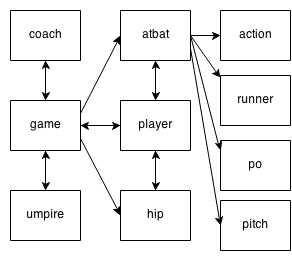
\includegraphics[scale = 0.75]{Drawing1.png}}

\caption{Table relations between Gameday data accessible via \code{scrape}.
The direction of the arrows indicate a one to possibly many relationship.
\label{fig:relations}}


\end{figure}



\section[{Introducing XML2R]{Introducing \pkg{XML2R}}

\pkg{XML2R} adds to the \href{http://cran.r-project.org/web/views/WebTechnologies.html}{CRAN Task View on Web Technologies and Services}
by focusing on the transformation of XML content into a collection
of tables. Compared to a lower-level API like the \pkg{XML} package,
it can significantly reduce the amount of coding and cognitive effort
required to perform such a task. In contrast to most higher-level
APIs, it does not make assumptions about the XML structure or its
source. Although \pkg{XML2R} works on any structure, performance
and user experience are enhanced if the content has an inherent relational
structure. \pkg{XML2R}'s novel approach to XML data collection breaks
down the transformation process into a few simple steps and allows
the user to decide how to apply those steps.

The next few sections demonstrate how \pkg{pitchRx} leverages \pkg{XML2R}
in order to produce a collection of tables from \code{inning\_all.xml}
files. A similar approach is used by \code{pitchRx::scrape} to construct
tables from the other Gameday files in Table~\ref{table:pitchfx}.
In fact, \pkg{XML2R} has also been implemented in the R package \href{https://github.com/cpsievert/bbscrapeR}{bbscrapeR}
which collects data from \href{http://nba.com}{nba.com} and \href{http://wnba.com}{wnba.com}.


\subsection{Constructing file names}

Sometimes the most frustrating part of obtaining data in bulk off
of the web is finding the proper collection of URLs or file names
of interest. Since files on the Gameday website are fairly well organized,
the \code{makeUrls} function can be used to construct \code{urls}
that point to every game's homepage within a window of dates.

%
\begin{Schunk}
\begin{Sinput}
urls <- makeUrls(start = "2011-06-01", end = "2011-06-01") 
sub("http://gd2.mlb.com/components/game/mlb/", "", head(urls))
\end{Sinput}
\begin{Soutput}
[1] "year_2011/month_06/day_01/gid_2011_06_01_anamlb_kcamlb_1"
[2] "year_2011/month_06/day_01/gid_2011_06_01_balmlb_seamlb_1"
[3] "year_2011/month_06/day_01/gid_2011_06_01_chamlb_bosmlb_1"
[4] "year_2011/month_06/day_01/gid_2011_06_01_clemlb_tormlb_1"
[5] "year_2011/month_06/day_01/gid_2011_06_01_colmlb_lanmlb_1"
[6] "year_2011/month_06/day_01/gid_2011_06_01_flomlb_arimlb_1"
\end{Soutput}
\end{Schunk}



\subsection{Extracting observations}

Once we have a collection of XML \code{files}, the next step is to
parse the content into a list of \dfn{observations}. An observation
is technically defined as a matrix with one row and some number of
columns. The columns are defined by XML attributes and the XML value
(if any) for a particular XML lineage. The name of each observation
tracks the XML hierarchy so observations can be grouped together in
a sensible fashion at a later point.

%
\begin{Schunk}
\begin{Sinput}
library(XML2R)
files <- paste0(urls, "/inning/inning_all.xml")
obs <- XML2Obs(files, url.map = TRUE, quiet = TRUE) 
table(names(obs))
\end{Sinput}
\begin{Soutput}

                               game                        game//inning 
                                 15                                 137 
       game//inning//bottom//action         game//inning//bottom//atbat 
                                116                                 532 
 game//inning//bottom//atbat//pitch     game//inning//bottom//atbat//po 
                               1978                                  61 
game//inning//bottom//atbat//runner           game//inning//top//action 
                                373                                 150 
           game//inning//top//atbat     game//inning//top//atbat//pitch 
                                593                                2183 
       game//inning//top//atbat//po    game//inning//top//atbat//runner 
                                 75                                 509 
                            url_map 
                                  1 
\end{Soutput}
\end{Schunk}


This output tells us that 1978
pitches were thrown in the bottom inning and 2183
were thrown in the top inning on June 1st, 2011. Also, there are 12
different levels of observations. The list element named \code{url\_map}
is not considered an observation and was included since \code{url.map = TRUE}.
This helps avoid repeating long file names in the \code{url\_key}
column which tracks the mapping between observations and file names. 

%
\begin{Schunk}
\begin{Sinput}
obs[c(1, 2500)]
\end{Sinput}
\begin{Soutput}
$`game//inning//top//atbat//pitch`
     des             id  type tfs      tfs_zulu               x        y       
[1,] "Called Strike" "3" "S"  "161107" "2011-06-01T20:11:07Z" "103.00" "149.38"
     sv_id           start_speed end_speed sz_top sz_bot pfx_x   pfx_z 
[1,] "110601_151108" "94.0"      "86.1"    "2.85" "1.36" "-8.12" "11.0"
     px       pz      x0       y0     z0      vx0     vy0        vz0     
[1,] "-0.143" "2.376" "-2.435" "50.0" "5.831" "9.058" "-137.334" "-7.288"
     ax        ay       az        break_y break_angle break_length pitch_type
[1,] "-15.446" "31.474" "-11.175" "23.8"  "46.3"      "4.0"        "FT"      
     type_confidence zone nasty spin_dir  spin_rate  cc mt url_key
[1,] ".909"          "2"  "39"  "216.336" "2753.789" "" "" "url1" 

$`game//inning//bottom//atbat//runner`
     id       start end  event         url_key
[1,] "471083" "2B"  "3B" "Field Error" "url6" 
\end{Soutput}
\end{Schunk}



\subsection{Renaming observations}

Before grouping observations into a collection tables based on their
names, one may want to \code{re\_name} observations. Observations
with names \code{'game//inning//bottom//atbat'} and \code{'game//inning//top//atbat'}
should be included in the same table since they share XML attributes
(in other words, the observations share variables). 

%
\begin{Schunk}
\begin{Sinput}
tmp <- re_name(obs, equiv = c("game//inning//top//atbat",                             
  "game//inning//bottom//atbat"), diff.name = "inning_side") 
\end{Sinput}
\end{Schunk}


By passing these names to the \code{equiv} argument, \code{re\_name}
determines the difference in the naming scheme and suppresses that
difference. In other words, observation names that match the \code{equiv}
argument will be renamed to \code{'game//inning//atbat'}. The information
removed from the name is not lost; however, as a new column is appended
to the end of each relevant observation. For example, notice how the
\code{inning\_side} column contains the part of the name we just
removed:

%
\begin{Schunk}
\begin{Sinput}
tmp[grep("game//inning//atbat", names(tmp))][1:2]
\end{Sinput}
\begin{Soutput}
$`game//inning//atbat`
     num b   s   o   start_tfs start_tfs_zulu         batter   stand b_height
[1,] "1" "3" "2" "0" "161034"  "2011-06-01T20:10:34Z" "430947" "L"   "5-10"  
     pitcher  p_throws
[1,] "462956" "R"     
     des                                                                     
[1,] "Erick Aybar singles on a line drive to center fielder Melky Cabrera.  "
     event    url_key inning_side
[1,] "Single" "url1"  "top"      

$`game//inning//atbat`
     num b   s   o   start_tfs start_tfs_zulu         batter   stand b_height
[1,] "2" "2" "3" "1" "161412"  "2011-06-01T20:14:12Z" "110029" "L"   "6-0"   
     pitcher  p_throws des                                    event      
[1,] "462956" "R"      "Bobby Abreu called out on strikes.  " "Strikeout"
     url_key inning_side
[1,] "url1"  "top"      
\end{Soutput}
\end{Schunk}


For similar reasons, other observation name pairs are renamed in a
similar fashion.

%
\begin{Schunk}
\begin{Sinput}
tmp <- re_name(tmp, equiv = c("game//inning//top//atbat//runner",                             
  "game//inning//bottom//atbat//runner"), diff.name = "inning_side")
tmp <- re_name(tmp, equiv = c("game//inning//top//action",                             
  "game//inning//bottom//action"), diff.name = "inning_side")  
tmp <- re_name(tmp, equiv = c("game//inning//top//atbat//po",                            
  "game//inning//bottom//atbat//po"), diff.name = "inning_side")
obs2 <- re_name(tmp, equiv = c("game//inning//top//atbat//pitch",                             
  "game//inning//bottom//atbat//pitch"), diff.name = "inning_side") 
table(names(obs2))
\end{Sinput}
\begin{Soutput}

                       game                game//inning 
                         15                         137 
       game//inning//action         game//inning//atbat 
                        266                        1125 
 game//inning//atbat//pitch     game//inning//atbat//po 
                       4161                         136 
game//inning//atbat//runner                     url_map 
                        882                           1 
\end{Soutput}
\end{Schunk}



\subsection{Linking observations}

After all that renaming, we now have 7
different levels of observations. Let's examine the first three observations
on the \code{game//inning} level:

%
\begin{Schunk}
\begin{Sinput}
obs2[grep("^game//inning$", names(obs2))][1:3] 
\end{Sinput}
\begin{Soutput}
$`game//inning`
     num away_team home_team next url_key
[1,] "1" "ana"     "kca"     "Y"  "url1" 

$`game//inning`
     num away_team home_team next url_key
[1,] "2" "ana"     "kca"     "Y"  "url1" 

$`game//inning`
     num away_team home_team next url_key
[1,] "3" "ana"     "kca"     "Y"  "url1" 
\end{Soutput}
\end{Schunk}


Before grouping observations into tables, it is usually important
preserve the parent-to-child relationships in the XML lineage. For
example, one may want to map a particular pitch back to the inning
in which it was thrown. Using the \code{add\_key} function, the relevant
value of \code{num} for \code{game//inning} observations can be
\code{recycle}d to its XML descendants.

%
\begin{Schunk}
\begin{Sinput}
obswkey <- add_key(obs2, parent = "game//inning", recycle = "num", key.name = "inning")
\end{Sinput}
\begin{Soutput}
A key for the following children will be generated for the game//inning node:
game//inning//atbat//pitch
game//inning//atbat//runner
game//inning//atbat
game//inning//action
game//inning//atbat//po
\end{Soutput}
\end{Schunk}


As it turns out, the \code{away\_team} and \code{home\_team} columns
are redundant as this information is embedded in the \code{url} column.
Thus, there is only one other informative attribute on this level
which is \code{next}. By recycling this value among its descendants,
we remove any need to retain a \code{game//inning} table.

%
\begin{Schunk}
\begin{Sinput}
obswkey <- add_key(obswkey, parent = "game//inning", recycle = "next")
\end{Sinput}
\begin{Soutput}
A key for the following children will be generated for the game//inning node:
game//inning//atbat//pitch
game//inning//atbat//runner
game//inning//atbat
game//inning//action
game//inning//atbat//po
\end{Soutput}
\end{Schunk}


It is also imperative that we can link a \code{pitch}, \code{runner},
or \code{po} back to a particular \code{atbat}. This can be done
as follows:

%
\begin{Schunk}
\begin{Sinput}
obswkey <- add_key(obswkey, parent = "game//inning//atbat", recycle = "num")
\end{Sinput}
\begin{Soutput}
A key for the following children will be generated for the game//inning//atbat node:
game//inning//atbat//pitch
game//inning//atbat//runner
game//inning//atbat//po
\end{Soutput}
\end{Schunk}



\subsection{Collapsing observations}

Finally, we are in a position to pool together observations that have
a common name. The \code{collapse\_obs} function achieves this by
row binding observations with the same name together and returning
a list of matrices. Note that \code{collapse\_obs} does not require
that observations from the same level to have the same set of variables
in order to be bound into a common table. In the case where variables
are missing, \code{NA}s will be inserted as values.

%
\begin{Schunk}
\begin{Sinput}
tables <- collapse_obs(obswkey) 
#As mentioned before, we do not need the 'inning' table 
tables <- tables[-grep("^game//inning$", names(tables))]      
table.names <- c("game", "action", "atbat", "pitch", "po", "runner") 
tables <- setNames(tables, table.names) 
head(tables[["runner"]])
\end{Sinput}
\begin{Soutput}
     id       start end  event                url_key inning_side inning next
[1,] "430947" ""    "1B" "Single"             "url1"  "top"       "1"    "Y" 
[2,] "430947" "1B"  "2B" "Stolen Base 2B"     "url1"  "top"       "1"    "Y" 
[3,] "430947" "2B"  "3B" "Groundout"          "url1"  "top"       "1"    "Y" 
[4,] "430947" "3B"  ""   "Groundout"          "url1"  "top"       "1"    "Y" 
[5,] "543333" ""    "1B" "Single"             "url1"  "bottom"    "1"    "Y" 
[6,] "543333" "1B"  ""   "Pickoff Attempt 1B" "url1"  "bottom"    "1"    "Y" 
     num score rbi earned
[1,] "1" NA    NA  NA    
[2,] "2" NA    NA  NA    
[3,] "3" NA    NA  NA    
[4,] "4" NA    NA  NA    
[5,] "7" NA    NA  NA    
[6,] "8" NA    NA  NA    
\end{Soutput}
\end{Schunk}



\section[{Collecting Gameday data with pitchRx]{Collecting Gameday data with \pkg{pitchRx}}

The main scraping function in \pkg{pitchRx}, \code{scrape}, can
be used to easily obtain data from the files listed in Table~\ref{table:pitchfx}.
In fact, any combination of these files can be queried using the \code{suffix}
argument. In the example below, the \code{start} and \code{end}
arguments are also used so that all available file types for June
1st, 2011 are queried.

%
\begin{Schunk}
\begin{Sinput}
library(pitchRx)
files <- c("inning/inning_all.xml", "inning/inning_hit.xml", 
  "miniscoreboard.xml", "players.xml")
dat <- scrape(start = "2011-06-01", end = "2011-06-01", suffix = files)
\end{Sinput}
\end{Schunk}


The \code{game.ids} option can be used instead of \code{start} and
\code{end} to obtain an equivalent \code{dat} object. This option
can be useful if the user wants to query specific games rather than
all games played over a particular time span. When using this \code{game.ids}
option, the built-in \code{gids} object, is quite convenient.

%
\begin{Schunk}
\begin{Sinput}
data(gids, package = "pitchRx")
gids11 <- gids[grep("2011_06_01", gids)]
head(gids11)
\end{Sinput}
\begin{Soutput}
[1] "gid_2011_06_01_anamlb_kcamlb_1" "gid_2011_06_01_balmlb_seamlb_1"
[3] "gid_2011_06_01_chamlb_bosmlb_1" "gid_2011_06_01_clemlb_tormlb_1"
[5] "gid_2011_06_01_colmlb_lanmlb_1" "gid_2011_06_01_flomlb_arimlb_1"
\end{Soutput}
\end{Schunk}


%
\begin{Schunk}
\begin{Sinput}
dat <- scrape(game.ids = gids11, suffix = files)
\end{Sinput}
\end{Schunk}


The object \code{dat} is a list of data frames containing all data
available for June 1st, 2011 using \code{scrape}. The list names
match the table names provided in Table~\ref{table:pitchfx}. For
example, \code{dat\$atbat} is data frame with every at bat on June
1st, 2011 and \code{dat\$pitch} has information related to the outcome
of each pitch (including PITCHf/x parameters). The \code{object.size}
of \code{dat} is nearly 300MB. Multiplying this number by 100 days
exceeds the RAM limitations on most machines. Thus, if a large amount
of data is required, the user should exploit the R database interface
\citep{DBI}.


\section{Storing and querying Gameday data}

Since PITCHf/x data can easily exhaust random-access memory, one should
consider establishing a database instance before using \code{scrape}.
By passing a database connection to the \code{connect} argument,
\code{scrape} will try to create (and/or append to existing) tables
using that connection. If the connection fails for some reason, tables
will be written as csv files in the current working directory. The
benefits of using the \code{connect} argument includes improved memory
management which can greatly reduce run time. \code{connect} will
support a MySQL connection, but creating a SQLite database is quite
easy with \CRANpkg{dplyr} \citep{dplyr}. 

%
\begin{Schunk}
\begin{Sinput}
library(dplyr)
my_db <- src_sqlite("GamedayDB.sqlite3", create = TRUE)
# Collect and store all PITCHf/x data from 2008 to 2013
scrape(start = "2008-01-01", end = "2014-01-01", 
  suffix = "inning/inning_all.xml", connect = my_db$con)
\end{Sinput}
\end{Schunk}


In the later sections, animations of four-seam and cut fastballs thrown
by Mariano Rivera and Phil Hughes during the 2011 season are created.
In order to obtain the necessary data, one must set criteria on: values
of the \code{pitcher\_name} field in the \code{pitch} table, values
of the \code{des} field in the \code{atbat} table, and the \code{url}
field in both tables. Thus, to speed the time to execute such a query,
one should create an index on these three fields.

%
\begin{Schunk}
\begin{Sinput}
dbSendQuery(my_db$con, "CREATE INDEX url_atbat ON atbat(url)") 
dbSendQuery(my_db$con, "CREATE INDEX url_pitch ON pitch(url)") 
dbSendQuery(my_db$con, "CREATE INDEX pitcher_index ON atbat(pitcher_name)") 
dbSendQuery(my_db$con, "CREATE INDEX des_index ON pitch(des)")
\end{Sinput}
\end{Schunk}


Although our desired query could be expressed entirely in SQL, \pkg{dplyr}'s
grammar for data manipulation (which is database agnostic) can help
to simplify the task. First, create \code{pitch11} and \code{atbat11}
which are \emph{representations} of 2011 data in \code{my\_db}.
That is, \code{pitch11} does not actually pull data from every pitch
from 2011 into memory, but is a portrayal of the relevant data sitting
in \code{my\_db}.

%
\begin{Schunk}
\begin{Sinput}
pitch11 <- tbl(my_db, sql("SELECT * FROM pitch WHERE pitch.url LIKE '%year_2011%'"))
atbat11 <- tbl(my_db, sql("SELECT * FROM atbat WHERE atbat.url LIKE '%year_2011%'"))
\end{Sinput}
\end{Schunk}


Next, \code{filter} the \code{atbat11} table to restrict to at bats
in 2011 where either Rivera or Hughes was the pitcher. Then \code{filter}
the \code{pitch11} table to include only four-seam (FF) and cut (FC)
fastballs from 2011. By taking an \code{inner\_join} of these two
filtered tables, we are left with one table representing the data
of interest. Lastly, \code{collect} the resulting database query
in order to bring the relevant data into the R session.

%
\begin{Schunk}
\begin{Sinput}
bats <- filter(atbat11, 
  pitcher_name == "Mariano Rivera" | pitcher_name == "Phil Hughes")
FBs <- filter(pitch11, pitch_type == "FF" | pitch_type == "FC")
pitches <- collect(inner_join(FBs, bats))
\end{Sinput}
\end{Schunk}



\section{Visualizing PITCHf/x}


\subsection{Strike-zone plots and umpire bias}

Amongst the most common PITCHf/x graphics are strike-zone plots. Such
a plot has two axes and the coordinates represent the location of
baseballs as they cross home plate. The term strike-zone plot can
refer to either \emph{density} or \emph{probabilistic} plots. Density
plots are useful for exploring what \emph{actually} occurred, but
probabilistic plots can help address much more interesting questions
using statistical inference. Although probabilistic plots can be used
to visually track any event probability across the strike-zone, their
most popular use is for addressing umpire bias in a strike versus
ball decision \citet{bias}. The probabilistic plots section demonstrates
how \pkg{pitchRx} simplifies the process behind creating such plots
via a case study on the impact of home field advantage on umpire decisions.

In the world of sports, it is a common belief that umpires (or referees)
have a tendency to favor the home team. PITCHf/x provides a unique
opportunity to add to this discussion by modeling the probability
of a called strike at home games versus away games. Specifically,
conditioned upon the umpire making a decision at a specific location
in the strike-zone, if the probability that a home pitcher receives
a called strike is higher than the probability that an away pitcher
receives a called strike, then there is evidence to support umpire
bias towards a home pitcher.

There are many different possible outcomes of each pitch, but we can
condition on the umpire making a decision by limiting to the following
two cases. A \dfn{called strike} is an outcome of a pitch where the
batter does not swing and the umpire declares the pitch a strike (which
is a favorable outcome for the pitcher). A \dfn{ball} is another
outcome where the batter does not swing and the umpire declares the
pitch a ball (which is a favorable outcome for the batter). All \code{decisions}
made starting in 2008 can be obtained from \code{my\_db} with the
following query using \pkg{dplyr}.

%
\begin{Schunk}
\begin{Sinput}
pitch <- select(tbl(my_db, "pitch"), px, pz, des)
atbat <- select(tbl(my_db, "atbat"), b_height, p_throws, stand, inning_side)
decisions <- collect(inner_join(pitch, atbat))
#This indicator is used as a response when constructing probabilistic plots
decisions$strike <- as.numeric(decisions$des %in% "Called Strike")
\end{Sinput}
\end{Schunk}



\subsubsection{Density plots}

The \code{decisions} data frame contains data on over 2.5 million
pitches thrown from 2008 to 2013. About a third of them are called
strikes and two-thirds balls. Figure~\ref{fig:STRIKES} shows the
density of all called strikes. Clearly, most called strikes occur
on the outer region of the strike-zone. Many factors could contribute
to this phenomenon; which we will not investigate here.

%
\begin{Schunk}
\begin{Sinput}
#strikeFX uses the stand variable to calculate strike-zones 
#Here is a slick way to create better labels for stand without changing its values
relabel <- function(variable, value) { 
  value <- sub("^R$", "Right-Handed Batter", value) 
  sub("^L$", "Left-Handed Batter", value) 
}
strikes <- subset(decisions, strike == 1)
strikeFX(strikes, geom = "tile", layer = facet_grid(. ~ stand, labeller = relabel))
\end{Sinput}
\end{Schunk}


\begin{figure}[h]
\centerline{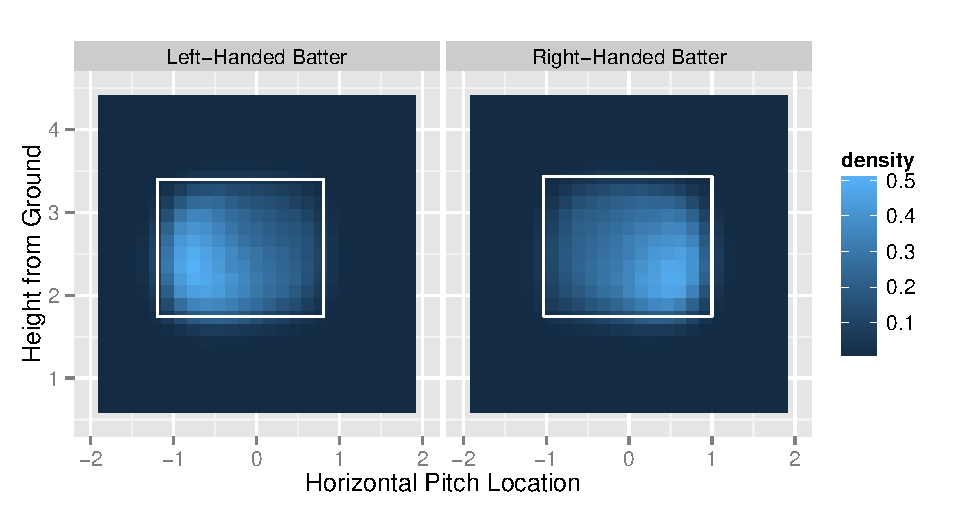
\includegraphics[scale = 1]{strikes.pdf}}

\caption{\label{fig:STRIKES} Density of called strikes for right-handed batters
and left-handed batters (from 2008 to 2013).}
\end{figure}


Figure~\ref{fig:STRIKES} shows one static rectangle (or strike-zone)
per plot automatically generated by \code{strikeFX}. The definition
of the strike-zone is notoriously ambiguous. As a result, the boundaries
of the strike-zone may be noticeably different in some situations.
However, we can achieve a fairly accurate representation of strike-zones
using a rectangle defined by batters' average height and stance \citep{Strikezones}.
As Figure~\ref{fig:strike-probs} reinforces, batter stance makes
an important difference since the strike-zone seems to be horizontally
shifted away from the batter. The batter's height is also important
since the strike-zone is classically defined as approximately between
the batter's knees and armpits.

Figure~\ref{fig:STRIKES} has is one strike-zone per plot since the
\code{layer} option contains a \pkg{ggplot2} argument that facets
according to batter stance. Facet layers are a powerful tool for analyzing
PITCHf/x data because they help produce quick and insightful comparisons.
In addition to using the \code{layer} option, one can add layers
to a graphic returned by \code{strikeFX} using \pkg{ggplot2} arithmetic.
It is also worth pointing out that Figure~\ref{fig:STRIKES} could
have been created without introducing the \code{strikes} data frame
by using the \code{density1} and \code{density2} options. 

%
\begin{Schunk}
\begin{Sinput}
strikeFX(decisions, geom = "tile", density1 = list(des = "Called Strike"),          
  density2 = list(des = "Called Strike")) + facet_grid(. ~ stand, labeller = relabel)
\end{Sinput}
\end{Schunk}


In general, when \code{density1} and \code{density2} are identical,
the result is equivalent to subsetting the data frame appropriately
beforehand. More importantly, by specifying \emph{different} values
for \code{density1} and \code{density2}, differenced densities are
easily generated. In this case, a grid of density estimates for \code{density2}
are subtracted from the corresponding grid of density estimates for
\code{density1}. Note that the default \code{NULL} value for either
density option infers that the entire data set defines the relevant
density. Thus, if \code{density2} was \code{NULL} (when \code{density1 = list(des = 'Called Strike')}),
we would obtain the density of called strikes minus the density of
\emph{both} called strikes and balls. In Figure~\ref{fig:strikesVSballs},
we define \code{density1} as called strikes and define \code{density2}
as balls. As expected, we see positive density values (in blue) inside
the strike-zone and negative density values (in red) outside of the
strike-zone. 

%
\begin{Schunk}
\begin{Sinput}
strikeFX(decisions, geom = "tile", density1 = list(des = "Called Strike"), 
  density2 = list(des = "Ball"), layer = facet_grid(. ~ stand, labeller = relabel)) 
\end{Sinput}
\end{Schunk}


\begin{figure}[h]
\centerline{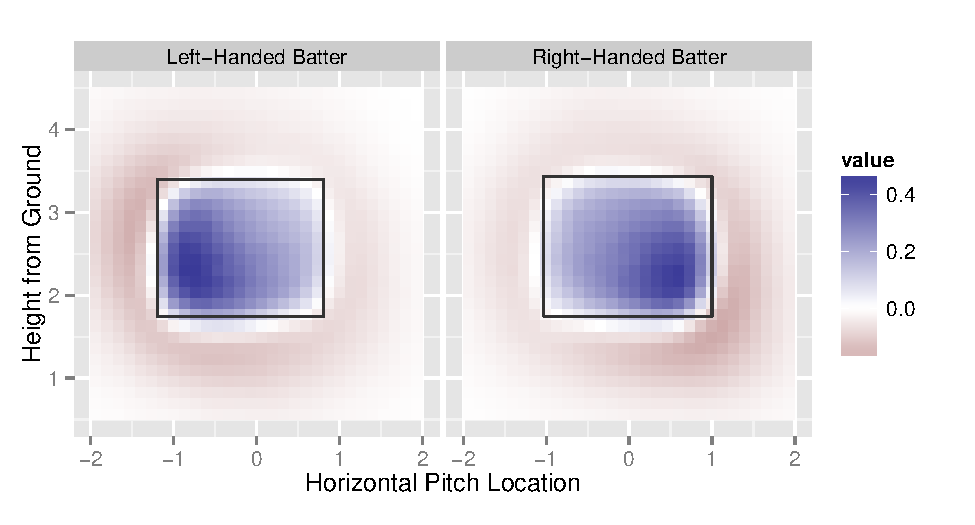
\includegraphics[scale = 1]{strikesVSballs.pdf}}

\caption{\label{fig:strikesVSballs} Density of called strikes minus density
of balls for both right-handed batters and left-handed batters (from
2008 to 2013). The blue region indicates a higher frequency of called
strikes and the red region indicates a higher frequency of balls.}
\end{figure}


These density plots are helpful for visualizing the observed frequency
of events; however, they are not very useful for addressing our umpire
bias hypothesis. Instead of looking simply at the \emph{density},
we want to model the \emph{probability} of a strike called at each
coordinate given the umpire has to make a decision. 


\subsubsection{Probabilistic plots}

There are many approaches to probabilistic modeling over a two dimensional
spatial region. Since our response is often categorical, generalized
additive models (GAMs) is a popular and desirable approach to modeling
events over the strike-zone \citep{loess}. There are numerous R package
implementations of GAMs, but the \code{bam} function from the \CRANpkg{mgcv}
package has several desirable properties \citep{mgcv}. Most importantly,
the smoothing parameter can be estimated using several different methods.
In order to have a reasonable estimate of the smooth 2D surface, GAMs
require fairly large amount of observations. As a result, run time
can be an issue -- especially when modeling 2.5 million observations!
Thankfully, the \code{bam} function has a \code{cluster} argument
which allows one to distribute computations across multiple cores
using the built in \pkg{parallel} package.

%
\begin{Schunk}
\begin{Sinput}
library(parallel) 
cl <- makeCluster(detectCores() - 1)
library(mgcv) 
m <- bam(strike ~ interaction(stand, p_throws, inning_side) +                
  s(px, pz, by = interaction(stand, p_throws, inning_side)),              
  data = decisions, family = binomial(link = 'logit'), cluster = cl)
\end{Sinput}
\end{Schunk}


This formula models the probability of a strike as a function of the
baseball's spatial location, the batter's stance, the pitcher's throwing
arm, and the side of the inning. Since home pitchers always pitch
during the top of the inning, \code{inning\_side} also serves as
an indication of whether a pitch is thrown by a home pitcher. In this
case, the \code{interaction} function creates a factor with eight
different levels since every input factor has two levels. Consequently,
there are 8 different levels of smooth surfaces over the spatial region
defined by \code{px} and \code{pz}.

The fitted model \code{m} contains a lot of information which \code{strikeFX}
uses in conjunction with any \pkg{ggplot2} facet commands to infer
which and how surfaces should be plotted. In particular, the \code{var.summary}
is used to identify model covariates, as well their default conditioning
values. In our case, the majority of \code{decisions} are from right-handed
pitchers and the top of the inning. Thus, the default conditioning
values are \code{"top"} for \code{inning\_side} and \code{"R"}
for \code{p\_throws}. If different conditioning values are desired,
\code{var.summary} can be modified accordingly. To demonstrate, Figure~\ref{fig:strike-probs}
shows 2 of the 8 possible surfaces that correspond to a right-handed
\emph{away} pitcher.

%
\begin{Schunk}
\begin{Sinput}
away <- list(inning_side = factor("bottom", levels = c("top", "bottom")))
m$var.summary <- modifyList(m$var.summary, away)
strikeFX(decisions, model = m, layer = facet_grid(. ~ stand, labeller = relabel))
\end{Sinput}
\end{Schunk}


\begin{figure}[h]
\centerline{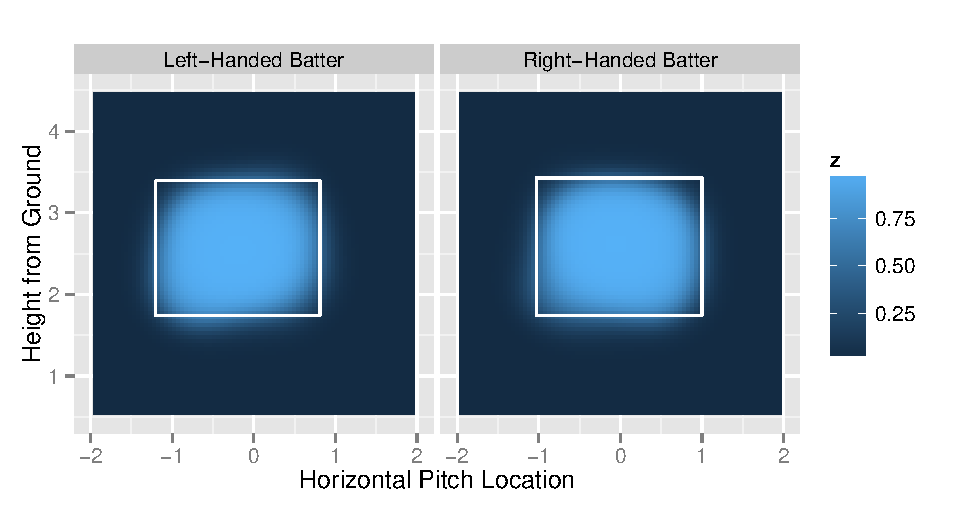
\includegraphics[scale = 1]{prob-strike.pdf}}

\caption{\label{fig:strike-probs}Probability that a right-handed away pitcher
receives a called strike (provided the umpire has to make a decision).
Plots are faceted by the handedness of the batter.}
\end{figure}


Using the same intuition exploited earlier to obtain differenced density
plots, we can easily obtain differenced probability plots. To obtain
Figure~\ref{fig:diff-probs}, we simply add \code{p\_throws} as
another facet variable and \code{inning\_side} as a differencing
variable. In this case, conditioning values do not matter since every
one of the 8 surfaces are required in order to produce Figure~\ref{fig:diff-probs}.

%
\begin{Schunk}
\begin{Sinput}
#function to create better labels for both stand and p_throws
relabel2 <- function(variable, value) {    
  if (variable %in% "stand")      
    return(sub("^L$", "Left-Handed Batter",                 
    sub("^R$", "Right-Handed Batter", value)))   
  if (variable %in% "p_throws")      
    return(sub("^L$", "Left-Handed Pitcher",                 
    sub("^R$", "Right-Handed Pitcher", value))) 
}
strikeFX(decisions, model = m, layer = facet_grid(p_throws ~ stand, labeller = relabel2),
  density1 = list(inning_side = "top"), density2 = list(inning_side = "bottom"))
\end{Sinput}
\end{Schunk}


\begin{figure}[h]
\centerline{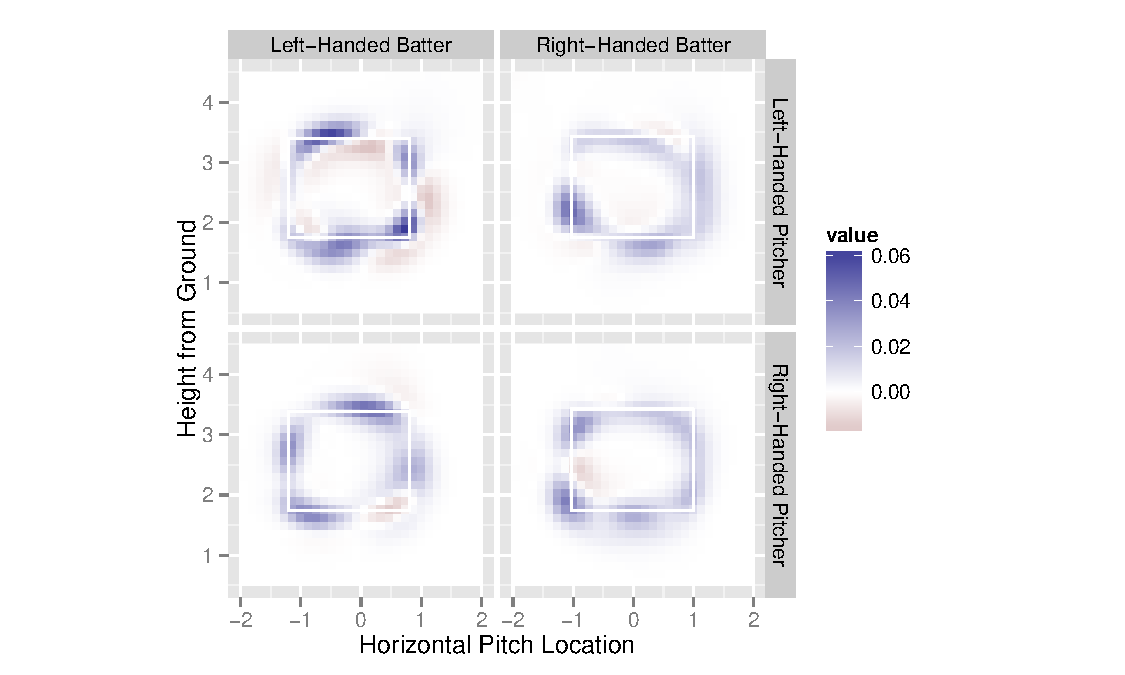
\includegraphics[scale = 1]{prob-diff.pdf}}

\caption{\label{fig:diff-probs}Difference between home and away pitchers in
the probability of a strike (provided the umpire has to make a decision).
The blue regions indicate a higher probability of a strike for home
pitchers and red regions indicate a higher probability of a strike
for away pitchers. Plots are faceted by the handedness of both the
pitcher and the batter.}
\end{figure}


The four different plots in Figure~\ref{fig:diff-probs} represent
the four different combination of values among \code{p\_throws} and
\code{stand}. In general, provided that a pitcher throws to a batter
in the blue region, the pitch is more likely to be called a strike
if the pitcher is on their home turf. Interestingly, there is a well-defined
blue elliptical band around the boundaries of the typical strike-zone.
Thus, home pitchers are more likely to receive a favorable call --
especially when the classification of the pitch is in question. In
some areas, the home pitcher has up to a 6 percent higher probability
of receiving a called strike than an away pitcher. The subtle differences
in spatial patterns across the different values of \code{p\_throws}
and \code{stand} are interesting as well. For instance, pitching
at home has a large positive impact for a left-handed pitcher throwing
in the lower inside portion of the strike-zone to a right-handed batter,
but the impact seems negligible in the mirror opposite case.

Differenced probabilistic densities are clearly an interesting visual
tool for analyzing PITCHf/x data. With \code{strikeFX}, one can quickly
and easily make all sorts of visual comparisons for various situations.
In fact, one can explore and compare the probabilistic structure of
any well-defined event over a strike-zone region (for example, the
probability a batter reaches base) using a similar approach. 


\subsection{2D animation}

\code{animateFX} provides convenient and flexible functionality for
animating the trajectory of any desired set of pitches. For demonstration
purposes, this section animates every four-seam and cut fastball thrown
by Mariano Rivera and Phil Hughes during the 2011 season. These pitches
provide a good example of how facets play an important role in extracting
new insights. Similar methods can be used to analyze any MLB player
(or combination of players) in greater detail.

\code{animateFX} tracks three dimensional pitch locations over a
sequence of two dimensional plots. The animation takes on the viewpoint
of the umpire; that is, each time the plot refreshes, the balls are
getting closer to the viewer. This is reflected with the increase
in size of the points as the animation progresses. Obviously, some
pitches travel faster than others, which explains the different sizes
within the same frame. Note that animations in this paper revert to
the initial point of release once \emph{all} of the baseballs have
reached home plate. During an interactive session, \code{animateFX}
produces a series of plots that may not viewed easily. One option
available to the user is to wrap \code{animation::saveHTML} around
\code{animateFX} to view the animation in a browser with proper looping
controls \citep{animation}.

To reduce the time and thinking required to produce these animations,
\code{animateFX} has default settings for the geometry, color, opacity
and size associated with each plot. Any of these assumptions can be
altered - except for the point geometry. In order for animations to
work, a data frame with the appropriately named PITCHf/x parameters
(that is, x0, y0, z0, vx0, vy0, vz0, ax0, ay0 and az0) is required.
In Figure~\ref{fig:animate1}, every four-seam and cut fastball thrown
by Rivera and Hughes during the 2011 season is visualized using the
\code{pitches} data frame obtained earlier.




\begin{figure}[h]
%
\begin{Schunk}
\begin{Sinput}
animateFX(pitches, layer=list(theme_bw(), coord_equal(),
  facet_grid(pitcher_name~stand, labeller = relabel)))
\end{Sinput}

\animategraphics[width=1.05\textwidth,controls,loop,autoplay]{20}{figure/all}{1}{45}\end{Schunk}


\caption{\label{fig:animate1}Animation of every four-seam and cutting fastballs
thrown by NY Yankee pitchers Mariano Rivera and Phil Hughes during
the 2011 season. Pitches are faceted by pitcher and batting stance.
For instance, the top left plot portrays pitches thrown by Rivera
to left-handed batters. Animations are intentionally slower than real-time
for visual recognition and should be viewed within \protect\href{http://get.adobe.com/reader/}{Adobe Reader}
\citep{knitr}.}
\end{figure}


The upper right-hand plot of Figure~\ref{fig:animate1} (Rivera throwing
to right-handed batters) reveals the clearest pattern in flight trajectories.
Around the point of release, Rivera's two pitch types are hard to
distinguish. However, after a certain point, there is a very different
flight path among the two pitch types. Specifically, the drastic left-to-right
movement of the cut fastball is noticeably different from the slight
right-to-left movement of the four-seam fastball. In recent years,
cut fastballs have gained notoriety among the baseball community as
a coveted pitch for pitchers have at their disposal. This is largely
due to the difficulty that a batter has in distinguishing the cut
fastball from another fastball as the ball travels toward home plate.
Clearly, this presents an advantage for the pitcher since they can
use deception to reduce batter's ability to predict where the ball
will cross home plate. This deception factor combined with Rivera's
ability to locate his pitches explain his accolades as one of the
greatest pitchers of all time \citep{NYT}.

Although we see a clear pattern in Rivera's pitches, MLB pitchers
are hardly ever that predictable. Animating that many pitches for
another pitcher can produce a very cluttered graphic which is hard
to interpret (especially when many pitch types are considered). However,
we may still want to obtain an indication of pitch trajectory over
a set of many pitches. A way to achieve this is to average over the
PITCHf/x parameters to produce an overall sense of pitch type behavior
(via the \code{avg.by} option). Note that the facet variables are
automatically considered indexing variables. That is, in Figure~\ref{fig:animate2},
there are eight 'average' pitches since there are two pitch types,
two pitchers, and two types of batting stance.

\begin{figure}[h]
%
\begin{Schunk}
\begin{Sinput}
animateFX(pitches, avg.by = "pitch_types", layer = list(coord_equal(), theme_bw(),
  facet_grid(pitcher_name~stand, labeller = relabel)))
\end{Sinput}

\animategraphics[width=1.05\textwidth,controls,loop,autoplay]{20}{figure/avg}{1}{41}\end{Schunk}


\caption{\label{fig:animate2}Animation of 'average' four-seam and cutting
fastballs thrown by NY Yankee pitchers Mariano Rivera and Phil Hughes
during the 2011 season. PITCHf/x parameters are averaged over pitch
type, pitcher and batting stance. For instance, the bottom right plot
portrays an ``average four-seam'' and ``average cutter'' thrown
by Hughes to right-handed batters. Animations are intentionally slower
than real-time for visual recognition and should be viewed within
\protect\href{http://get.adobe.com/reader/}{Adobe Reader}.}
\end{figure}



\subsection{Interactive 3D graphics}

\pkg{rgl} is an R package that utilizes OpenGL for graphics rendering.
\code{interactiveFX} utilizes \pkg{rgl} functionality to reproduce
flight paths on an interactive 3D platform. Figure~\ref{fig:rgl}
has two static pictures of Mariano Rivera's 2011 fastballs on this
interactive platform. This is great for gaining new perspectives on
a certain set of pitches, since the trajectories can be viewed from
any angle. Figure~\ref{fig:rgl} showcases the difference in trajectory
between Rivera's pitch types.

%
\begin{Schunk}
\begin{Sinput}
Rivera <- subset(pitches, pitcher_name == "Mariano Rivera")
interactiveFX(Rivera, avg.by = "pitch_types")
\end{Sinput}
\end{Schunk}


\begin{figure}[h]
\begin{minipage}[t]{0.45\textwidth}%
\centerline{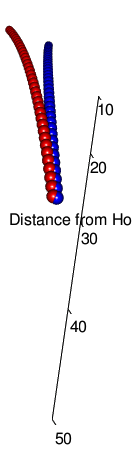
\includegraphics[scale = .45]{rgl_b.png}}%
\end{minipage}\hspace*{\fill}%
\begin{minipage}[t]{0.45\textwidth}%
\centerline{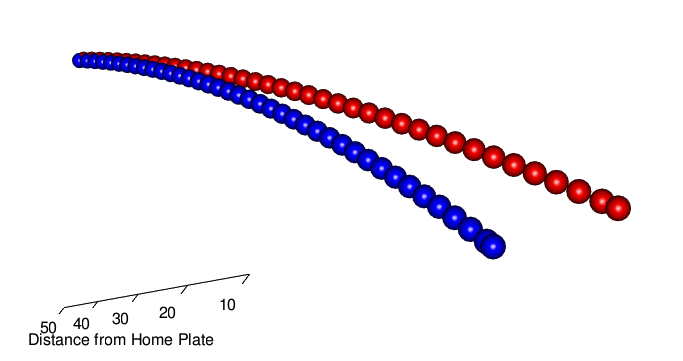
\includegraphics[scale = .45]{rgl_a.png}}%
\end{minipage}

\caption{3D scatterplot of pitches from Rivera. Pitches are plotted every one-hundredth
of a second. Cutting fastballs are shown in red and four-seam fastballs
are shown in blue. The left hand plot takes a viewpoint of Rivera
and the right hand plot takes a viewpoint near the umpire. Note these
are static pictures of an interactive object. \label{fig:rgl}}
\end{figure}



\section{Conclusion}

\pkg{pitchRx} utilizes \pkg{XML2R}'s convenient framework for manipulating
XML content in order to provide easy access to PITCHf/x and related
Gameday data. \pkg{pitchRx} removes access barriers which allows
the average R user and baseball fan to spend their valuable time analyzing
Gameday's enormous source of baseball information. \pkg{pitchRx}
also provides a suite of functions that greatly reduce the amount
of work involved to create popular PITCHf/x graphics. For those interested
in obtaining other XML data, \pkg{pitchRx} serves as a nice example
of leveraging \pkg{XML2R} to quickly assemble custom XML data collection
mechanisms.


\section{Acknowledgements}

Many thanks to my major professor, Dr. Heike Hofmann, for her direction
and support throughout this project. Thanks also to the anonymous
reviewers for helpful feedback.



bibliography{sievert}


\address{Carson Sievert\\
Department of Statistics\\
Iowa State University}\\
\email{sievert@iastate.edu}

\end{article}
